
% Approach and results with respect to the Boosting approach


\section{Boosting}
% Approach and results with respect to the Boosting approach
\subsection{Data Preprocessing}
AdaBoost was chosen as our boosting algorithm. The weak classifiers used were decision trees. Training data was processed by running each sample through a pre-trained deep sentence embedding model to produce a 384 dimensional dense vector. The embedding model used was \verb|all-MiniLM-L12-v2 | from the \verb|sentence-transformers| library provided by HuggingFace \cite{HuggingFace}, this was chosen for its strong listed transfer performance and its relatively small size. However, this model is optimised for sentences of 128 words or less and will truncate sentences that are longer. Because many of the reviews in the dataset are longer than 512 words this poses an issue. Experiments were performed using tokenisation and stop word removal to reduce sentence length but this severely worsened the performance of the model. This makes sense because the embedding model is trained on natural language and assumes input sentences are grammatical. Instead, any reviews longer than 128 words are split into 128 word long chunks which are embedded individually and averaged together. In order to preserve semantic continuity between chunks they overlap by 15 words. Chunks are weighted by length when averaged to account for reviews which are not a multiple of 128 long. This provided a significant improvement in accuracy, approximately 5\%,  over allowing long reviews to be truncated.

\subsection{Hyper-parameter Tuning}
Hyper-parameter tuning was done using grid search over the parameters \verb|max_depth|, which controls the maximum depth of the trees used as weak classifiers, and \verb|num_classifiers| which controls the total number of trees used. The range searched for \verb|num_classifiers| was $[50, 100, 200, 500]$ and the range of \verb|max_depth| was $[2, 5, 10, 25]$. It was only possible to search a small range of parameters because grid search scales in $O(n*m)$ time where $n$ and $m$ are the numbers of candidates for each hyper-parameter, and because training the model can take a long time, especially when using many deep trees. The performance of each model in the search space was assessed using 5-fold cross validation and the model with the best average accuracy was chosen as our final model. \autoref{fig:BoostTuning} shows the results of the grid search. There seems to be only a small different in model accuracy between models with different hyper-parameters. The final hyper-parameters chosen were \verb|num_classifiers = 100| and \verb|max_depth = 2|. This is because they achieved the best cross-validated accuracy. 

\begin{figure}
    \centering
    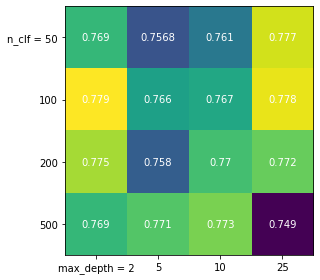
\includegraphics[width= 0.4\textwidth]{hyperparam_tuning_boosting.png}
    \caption{Hyper-parameter grid search for AdaBoost classifier}
    \label{fig:BoostTuning}
\end{figure}

\subsection{Analysis of misclassification}


\begin{figure}
    \centering
    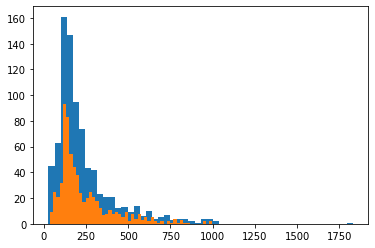
\includegraphics[width= 0.4\textwidth]{sections/Misclass_Lenghts.png}
    \caption{Lengths of correctly classified (blue) and misclassified (red) reviews.}
    \label{fig:MisclassLengths}
\end{figure}